% presentation.tex — 25-minute defense slides (English)
% Compile: tectonic presentation.tex
\documentclass[11pt,aspectratio=169]{beamer}

\usetheme{Madrid}
\usecolortheme{seahorse}

% ---- UPM identity colors (same as tfm.tex) ----
\definecolor{upmOrange}{HTML}{FF8000}
\definecolor{upmBlue}{HTML}{243F60}
\definecolor{tblAltRow}{HTML}{EDF1F7}
\definecolor{codebg}{rgb}{0.97,0.97,0.97}
\definecolor{codeblue}{rgb}{0.13,0.29,0.53}
\definecolor{codegreen}{rgb}{0.0,0.45,0.0}
\definecolor{codegray}{rgb}{0.5,0.5,0.5}

\setbeamercolor{palette primary}{bg=upmBlue,fg=white}
\setbeamercolor{palette secondary}{bg=upmBlue!85,fg=white}
\setbeamercolor{palette tertiary}{bg=upmBlue!70,fg=white}
\setbeamercolor{palette quaternary}{bg=upmBlue,fg=white}
\setbeamercolor{structure}{fg=upmBlue}
\setbeamercolor{frametitle}{bg=upmBlue,fg=white}
\setbeamercolor{title}{bg=upmBlue,fg=white}
\setbeamercolor{block title}{bg=upmOrange,fg=white}
\setbeamercolor{block body}{bg=upmOrange!8,fg=black}
\setbeamercolor{block title alerted}{bg=red!70!black,fg=white}
\setbeamercolor{block body alerted}{bg=red!5,fg=black}
\setbeamercolor{block title example}{bg=teal!70!black,fg=white}
\setbeamercolor{block body example}{bg=teal!5,fg=black}
\setbeamertemplate{navigation symbols}{}
\setbeamertemplate{blocks}[rounded][shadow=false]
\setbeamerfont{frametitle}{series=\bfseries}

\usepackage{tikz}
\usetikzlibrary{arrows.meta,positioning}
\usepackage{pgfplots}
\pgfplotsset{compat=1.17}
\usepackage{booktabs}
\usepackage{colortbl}
\usepackage{amsmath}
\usepackage{listings}
\usepackage{pifont}
\newcommand{\cmark}{\textcolor{codegreen}{\ding{51}}}
\newcommand{\xmark}{\textcolor{red!70!black}{\ding{55}}}

\lstset{
  basicstyle=\footnotesize\ttfamily,
  backgroundcolor=\color{codebg},
  keywordstyle=\color{codeblue}\bfseries,
  commentstyle=\color{codegray}\itshape,
  stringstyle=\color{codegreen},
  frame=single, rulecolor=\color{gray!40},
  language=Python, showstringspaces=false,
  breaklines=true,
}

% ---------------------------------------------------------------
\title[Dataset Quality \& Leakage Detection]{An Automated Framework for Dataset Quality Assessment and Data Leakage Detection in Machine Learning}
\subtitle{Master's Thesis Defense}
\author[Jaime Cano Moraño]{Jaime Cano Moraño}
\institute[UPM]{ETSIT --- Universidad Politécnica de Madrid \\ Illinois Institute of Technology}
\date{July 2026}

\begin{document}

% ============================================================ 1
\begin{frame}
  \titlepage
\end{frame}

% ============================================================ 2
\begin{frame}{The Problem: Models Fail Because of Data, Not Algorithms}
  \begin{itemize}\setlength\itemsep{0.6em}
    \item Most ML effort targets \textbf{models}; most production failures trace back to \textbf{data}: missing values, duplicates, imbalance, drift \ldots{} and, most insidiously, \textbf{data leakage}.
    \item \textbf{Data leakage}: information about the target reaches the training features in a way that will not exist at prediction time.
    \item Leakage is dangerous because it is \emph{silent}: the model looks \textbf{better}, not worse --- inflated validation metrics that collapse in production.
    \item Documented across medicine, finance, and academic reproducibility studies (Kaufman et al.\ 2012; Kapoor \& Narayanan).
  \end{itemize}
  \vspace{0.5em}
  \begin{block}{Core question of this thesis}
    Can dataset quality assessment and leakage detection be \textbf{automated, quantified, and made actionable} in a single tool?
  \end{block}
\end{frame}

% ============================================================ 3
\begin{frame}{A Motivating Example}
  A logistic regression classifier trained on a dataset with an engineered leaky feature:
  \vspace{0.8em}
  \begin{columns}[T]
    \begin{column}{0.48\textwidth}
      \begin{alertblock}{With leakage (as delivered)}
        \centering\Large Validation accuracy: \textbf{1.000}
      \end{alertblock}
    \end{column}
    \begin{column}{0.48\textwidth}
      \begin{exampleblock}{After removing leaky features}
        \centering\Large Validation accuracy: \textbf{0.952}
      \end{exampleblock}
    \end{column}
  \end{columns}
  \vspace{1.0em}
  \begin{itemize}\setlength\itemsep{0.5em}
    \item That $\Delta = -0.048$ is the gap between a reproducible result and a broken one.
    \item A human reviewer might catch this. \textbf{At scale, nobody reviews every feature of every dataset.}
    \item The framework presented today detects this automatically --- and quantifies the damage.
  \end{itemize}
\end{frame}

% ============================================================ 4
\begin{frame}{The Gap in Existing Tools}
  \begin{itemize}\setlength\itemsep{0.5em}
    \item Mature open-source tools exist for data \emph{profiling} and \emph{validation}:
      \textbf{ydata-profiling}, \textbf{Great Expectations}, \textbf{Deepchecks}.
    \item They cover descriptive statistics and rule-based validation well \ldots
    \item \ldots{} but \textbf{leakage detection is almost absent}: on four constructed leakage scenarios, they detect \textbf{at most 1 of 4} (and only via manually authored rules).
    \item None produces a single interpretable \emph{readiness} verdict or code-level fixes.
  \end{itemize}
  \vspace{0.6em}
  \begin{block}{Positioning}
    The framework \textbf{complements} these tools --- it fills the leakage-detection and
    actionability gap rather than replacing general-purpose profiling.
  \end{block}
\end{frame}

% ============================================================ 5
\begin{frame}{Objectives and Contributions}
  \begin{enumerate}\setlength\itemsep{0.8em}
    \item \textbf{A unified, automated framework}: 20 deterministic checks across 5 dimensions (quality, leakage, features, sufficiency, drift) + impact analysis, with CLI, Python SDK, and web interfaces.
    \item \textbf{A unified Leakage Risk Score} $\mathcal{L}(f)$ combining correlation, mutual information, and single-feature performance inflation into one flaggable number per feature.
    \item \textbf{LLM-based semantic leakage analysis}: detecting leakage from feature \emph{meaning} (e.g.\ \texttt{discharge\_date}) where statistics alone are blind.
    \item \textbf{A quantitative benchmark} against three widely used tools on a 29-item checklist and four leakage scenarios.
  \end{enumerate}
  \vspace{0.5em}
  \centering\footnotesize
  Validated on \textbf{12 datasets} (6 synthetic + 6 real-world) $\cdot$ \textbf{325 unit tests} $\cdot$ open source
\end{frame}

% ============================================================ 6
\begin{frame}{System Architecture}
  \centering
  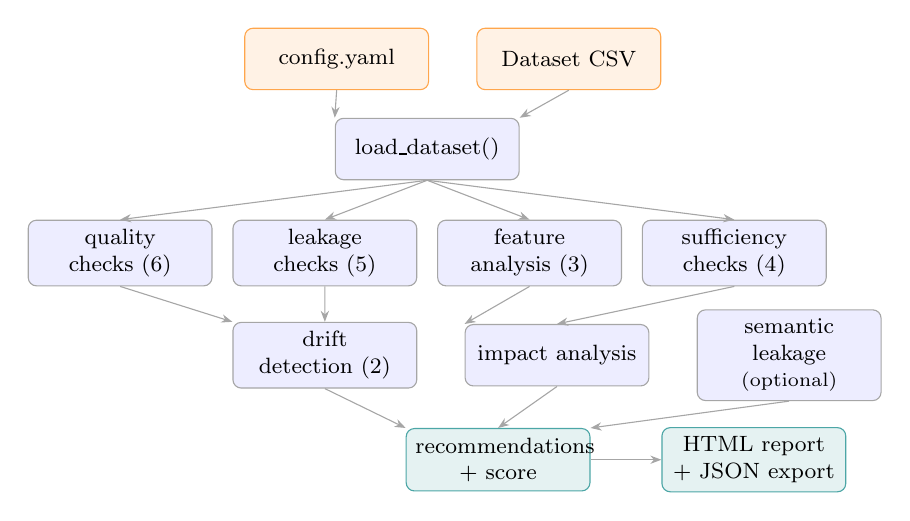
\begin{tikzpicture}[
    node distance=0.45cm and 0.9cm,
    box/.style={rectangle, rounded corners=3pt, draw=gray!70, fill=blue!7,
                 minimum height=0.78cm, minimum width=2.1cm,
                 font=\footnotesize, align=center, text width=2.1cm},
    outbox/.style={rectangle, rounded corners=3pt, draw=teal!70, fill=teal!10,
                 minimum height=0.78cm, minimum width=2.1cm,
                 font=\footnotesize, align=center, text width=2.1cm},
    io/.style={rectangle, rounded corners=3pt, draw=orange!70, fill=orange!10,
                 minimum height=0.78cm, minimum width=2.1cm,
                 font=\footnotesize, align=center, text width=2.1cm},
    arr/.style={-{Stealth[length=4pt]}, gray!70},
  ]
  \node[io]   (cfg)   {config.yaml};
  \node[io, right=0.6cm of cfg]  (data)  {Dataset CSV};
  \node[box, below=0.35cm of cfg, xshift=1.15cm] (load) {load\_dataset()};

  \node[box, below=0.5cm of load, xshift=-3.9cm] (qual)  {quality checks (6)};
  \node[box, below=0.5cm of load, xshift=-1.3cm] (leak)  {leakage checks (5)};
  \node[box, below=0.5cm of load, xshift=+1.3cm] (feat)  {feature analysis (3)};
  \node[box, below=0.5cm of load, xshift=+3.9cm] (suff)  {sufficiency checks (4)};

  \node[box, below=0.45cm of qual, xshift=2.6cm] (drift)  {drift\\detection (2)};
  \node[box, right=0.6cm of drift]  (impact) {impact analysis};
  \node[box, right=0.6cm of impact] (sem)    {semantic leakage \scriptsize(optional)};

  \node[outbox, below=0.5cm of drift, xshift=2.2cm] (rec)   {recommendations + score};
  \node[outbox, right=0.9cm of rec]                 (rep)   {HTML report + JSON export};

  \draw[arr] (cfg.south) -- (load.north west);
  \draw[arr] (data.south) -- (load.north east);
  \draw[arr] (load.south) -- (qual.north);
  \draw[arr] (load.south) -- (leak.north);
  \draw[arr] (load.south) -- (feat.north);
  \draw[arr] (load.south) -- (suff.north);
  \draw[arr] (qual.south) -- (drift.north west);
  \draw[arr] (leak.south) -- (drift.north);
  \draw[arr] (feat.south) -- (impact.north west);
  \draw[arr] (suff.south) -- (impact.north);
  \draw[arr] (drift.south) -- (rec.north west);
  \draw[arr] (impact.south) -- (rec.north);
  \draw[arr] (sem.south) -- (rec.north east);
  \draw[arr] (rec.east) -- (rep.west);
  \end{tikzpicture}

  \vspace{0.4em}
  \footnotesize One YAML config + one CSV in $\;\rightarrow\;$ 20 checks in 5 dimensions $\;\rightarrow\;$ recommendations, readiness score, and reports out.
\end{frame}

% ============================================================ 7
\begin{frame}[fragile]{Three Interfaces, One Pipeline}
  \begin{columns}[T]
    \begin{column}{0.42\textwidth}
      \begin{itemize}\setlength\itemsep{0.7em}
        \item \textbf{CLI} --- \texttt{main.py}: batch runs, CI/CD friendly.
        \item \textbf{Python SDK} --- \texttt{DatasetChecker}: notebooks and pipelines.
        \item \textbf{Streamlit web app} --- seven-tab interactive dashboard for non-programmers.
      \end{itemize}
      \vspace{0.5em}
      \footnotesize Plus a \texttt{@register\_check} \textbf{plugin API} for custom, domain-specific checks.
    \end{column}
    \begin{column}{0.56\textwidth}
\begin{lstlisting}
from src.checker import DatasetChecker

checker = DatasetChecker(
    "configs/config.yaml")
report = checker.run(
    "data/titanic.csv",
    target_col="survived")

print(checker.score, checker.grade)
checker.save_report("reports/")
\end{lstlisting}
    \end{column}
  \end{columns}
\end{frame}

% ============================================================ 8
\begin{frame}{The 20-Check Catalog (5 Dimensions)}
  \centering\small
  \begin{tabular}{llp{6.2cm}}
    \toprule
    \textbf{Dimension} & \textbf{\#} & \textbf{Checks} \\
    \midrule
    Quality      & 6 & missing values, duplicates, outliers, class imbalance, constant features, low variance \\
    \rowcolor{tblAltRow}
    Leakage      & 5 & target leakage, train/test overlap, temporal, ID columns, \textbf{unified risk score} \\
    Features     & 3 & correlation structure, MI relevance, distribution shape \\
    \rowcolor{tblAltRow}
    Sufficiency  & 4 & sample size, $n/p$ ratio, class support, power \\
    Drift        & 2 & KS test, PSI (covariate + label) \\
    \bottomrule
  \end{tabular}
  \vspace{0.8em}
  \begin{itemize}
    \item Each check returns a structured \texttt{CheckResult} (pass/fail, severity, affected columns).
    \item Failed checks map to \textbf{20 recommendation handlers} producing \emph{code-level} fixes.
    \item Optional 21st check: LLM semantic leakage (disabled by default).
  \end{itemize}
\end{frame}

% ============================================================ 9
\begin{frame}{Contribution: Unified Leakage Risk Score $\mathcal{L}(f)$}
  Single statistics miss real leaks; three signals combined are far more robust:
  \begin{equation*}
    \mathcal{L}(f) \;=\; 0.35\,\rho(f) \;+\; 0.35\,\tilde{I}(f;y) \;+\; 0.30\,\pi(f)
  \end{equation*}
  \vspace{-0.8em}
  \begin{itemize}\setlength\itemsep{0.4em}
    \item $\rho(f)$ --- Pearson $|r|$ (numeric) or Cramér's V (categorical) $\in [0,1]$
    \item $\tilde{I}(f;y)$ --- mutual information, normalized by the maximum MI $\in [0,1]$
    \item $\pi(f)$ --- \emph{single-feature performance inflation}: $\dfrac{A_f - A_{\text{base}}}{1 - A_{\text{base}}}$ --- how close does this one feature alone get a model to perfect accuracy?
  \end{itemize}
  \vspace{0.4em}
  \begin{block}{Flagging thresholds}
    $\mathcal{L}(f) \ge 0.7 \Rightarrow$ \textbf{warning} \qquad
    $\mathcal{L}(f) \ge 0.9 \Rightarrow$ \textbf{error}
  \end{block}
\end{frame}

% ============================================================ 10
\begin{frame}{Are the Weights Arbitrary? --- Ablation}
  Weight-sensitivity analysis on known leaky features (Titanic):
  \vspace{0.5em}
  \begin{center}\small
  \begin{tabular}{lcc}
    \toprule
    \textbf{Weight scheme} $(\rho/\tilde{I}/\pi)$ & $\mathcal{L}(\texttt{name})$ & $\mathcal{L}(\texttt{boat})$ \\
    \midrule
    \textbf{Default (0.35/0.35/0.30)} & \textbf{1.000} & \textbf{0.74 \cmark} \\
    \rowcolor{tblAltRow}
    Correlation-heavy (0.50/0.25/0.25) & 1.000 & 0.662 \xmark\; \footnotesize(below threshold!) \\
    MI- or $\pi$-weighted schemes & 1.000 & flagged \cmark \\
    \bottomrule
  \end{tabular}
  \end{center}
  \vspace{0.8em}
  \begin{itemize}\setlength\itemsep{0.5em}
    \item \texttt{boat} (lifeboat number) is a true leak, but its raw correlation is diluted by missing values --- an over-weighted correlation term produces a \textbf{false negative}.
    \item Every scheme that gives reasonable weight to MI or performance inflation catches it.
    \item Empirical evidence that the default weights are \emph{defensible}, not decorative.
  \end{itemize}
\end{frame}

% ============================================================ 11
\begin{frame}{Contribution: Semantic Leakage Analysis with an LLM}
  \begin{columns}[T]
    \begin{column}{0.52\textwidth}
      \textbf{Why statistics are not enough}
      \begin{itemize}\setlength\itemsep{0.5em}
        \item A feature named \texttt{discharge\_date} in an ICU mortality dataset is leaky \emph{by meaning}: it may show weak correlation, yet it cannot exist at prediction time.
        \item No statistical test reads feature \emph{names}.
      \end{itemize}
      \vspace{0.5em}
      \textbf{Approach}
      \begin{itemize}\setlength\itemsep{0.4em}
        \item Feature names + sample values + dataset description $\rightarrow$ \textbf{GPT-4o-mini} (Azure OpenAI).
        \item Degrades gracefully without credentials; disabled by default.
      \end{itemize}
    \end{column}
    \begin{column}{0.44\textwidth}
      \begin{block}{Per-feature output}
        \small
        \texttt{risk\_level}: none / low / medium / high \\[0.3em]
        \texttt{leakage\_type}: temporal / proxy / post-hoc / indirect \\[0.3em]
        + natural-language rationale
      \end{block}
      \vspace{0.4em}
      \footnotesize Raises naming-based leakage detection from \textbf{0\%} (no statistical signal) to \textbf{F1 = 0.963} on a 30-feature labelled benchmark.
    \end{column}
  \end{columns}
\end{frame}

% ============================================================ 12
\begin{frame}{Semantic Module: Evaluation and an Honest Caveat}
  \begin{itemize}\setlength\itemsep{0.6em}
    \item Manually labelled \textbf{30-feature benchmark} across temporal, proxy, post-hoc, and indirect leakage types (\texttt{data/semantic\_benchmark.json}).
    \item Results: \textbf{Precision = 1.00, Recall = 0.93, F1 = 0.963}.
  \end{itemize}
  \vspace{0.5em}
  \begin{alertblock}{Transparency}
    These figures validate the \textbf{evaluation harness} using a deterministic mock
    analyzer --- not the live GPT-4o-mini model (Azure credentials were unavailable at
    evaluation time). A live-model evaluation is the \textbf{top-priority item of future work},
    and this is stated explicitly in the thesis.
  \end{alertblock}
  \vspace{0.5em}
  \footnotesize The architecture, prompt design, structured output parsing, and graceful
  degradation are fully implemented and tested (33 unit tests for Phase 16 modules).
\end{frame}

% ============================================================ 13
\begin{frame}{From 20 Checks to One Number: the Readiness Score}
  \begin{equation*}
    \text{overall} \;=\; 0.25\,S_{\text{quality}} + \mathbf{0.35}\,S_{\text{leakage}} + 0.25\,S_{\text{features}} + 0.15\,S_{\text{sufficiency}}
  \end{equation*}
  \vspace{-0.6em}
  \begin{itemize}\setlength\itemsep{0.5em}
    \item Per dimension: start at 100, subtract \textbf{15 per error}, \textbf{5 per warning}.
    \item \textbf{Leakage carries the largest weight (0.35)}: it is the only failure mode that \emph{silently inflates} results instead of visibly degrading them.
    \item All weights and penalties are \textbf{configurable} in \texttt{config.yaml}.
  \end{itemize}
  \vspace{0.4em}
  \begin{center}
    \begin{tabular}{ccccc}
      \colorbox{codegreen!20}{\textbf{A} $\ge 85$} &
      \colorbox{teal!15}{\textbf{B} $\ge 70$} &
      \colorbox{orange!20}{\textbf{C} $\ge 55$} &
      \colorbox{orange!40}{\textbf{D} $\ge 40$} &
      \colorbox{red!20}{\textbf{F} $< 40$}
    \end{tabular}
  \end{center}
\end{frame}

% ============================================================ 14
\begin{frame}{Experimental Setup: 12 Datasets}
  \begin{columns}[T]
    \begin{column}{0.48\textwidth}
      \textbf{6 synthetic (controlled ground truth)}
      \begin{itemize}\small\setlength\itemsep{0.3em}
        \item \texttt{clean\_dataset} --- control
        \item \texttt{dirty\_dataset} --- quality issues
        \item \texttt{leaky\_dataset} --- leakage issues
        \item \texttt{proxy\_leakage} --- graded noisy proxies
        \item \texttt{temporal\_leakage\_ext} --- future feature
        \item \texttt{multitype\_leakage} --- ICU: proxy + temporal + ID
      \end{itemize}
    \end{column}
    \begin{column}{0.48\textwidth}
      \textbf{6 real-world (OpenML / UCI)}
      \begin{itemize}\small\setlength\itemsep{0.3em}
        \item Titanic (1{,}309 rows)
        \item Pima Diabetes (768)
        \item Adult Census (48{,}842)
        \item German Credit (1{,}000)
        \item Heart Disease (303)
        \item Wine Quality (1{,}599)
      \end{itemize}
    \end{column}
  \end{columns}
  \vspace{0.8em}
  \begin{itemize}
    \item Synthetic sets verify the framework \textbf{detects what we planted}; real sets verify it \textbf{finds surprises in the wild}.
    \item Full pipeline per dataset: 20 checks + impact analysis (23 results).
  \end{itemize}
\end{frame}

% ============================================================ 15
\begin{frame}{Results: Readiness Scores Discriminate as Designed}
  \centering
  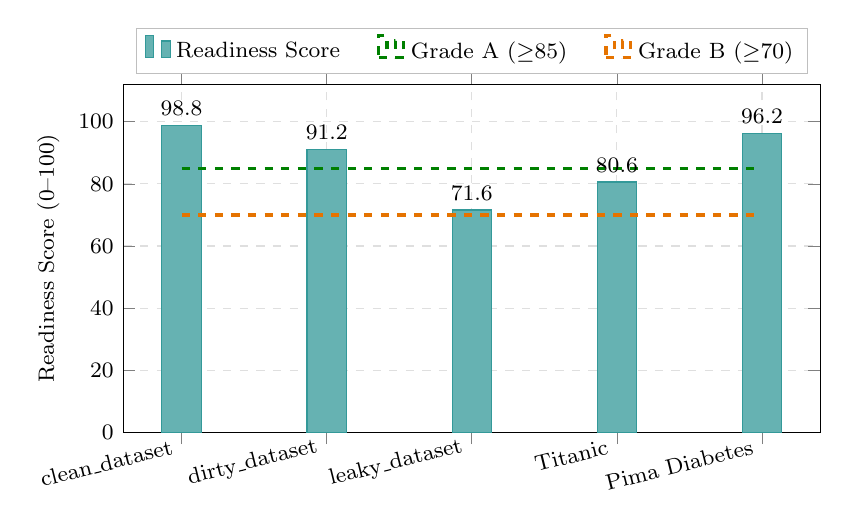
\begin{tikzpicture}
  \begin{axis}[
    ybar, width=0.86\textwidth, height=6.0cm, bar width=0.5cm,
    symbolic x coords={clean,dirty,leaky,Titanic,Diabetes},
    xtick=data,
    xticklabels={clean\_dataset, dirty\_dataset, leaky\_dataset, Titanic, Pima Diabetes},
    x tick label style={font=\footnotesize, rotate=14, anchor=east},
    ylabel={Readiness Score (0--100)}, ylabel style={font=\footnotesize},
    ymin=0, ymax=112, ytick={0,20,40,60,80,100},
    yticklabel style={font=\footnotesize},
    grid=major, grid style={dashed, gray!25},
    legend style={at={(0.5,1.03)}, anchor=south, font=\footnotesize,
                  draw=gray!50, fill=white, legend columns=-1,
                  /tikz/every even column/.append style={column sep=0.4cm}},
  ]
  \addplot[fill=teal!60, draw=teal!80,
           nodes near coords, every node near coord/.style={font=\footnotesize\bfseries}]
    coordinates {(clean,98.8)(dirty,91.2)(leaky,71.6)(Titanic,80.6)(Diabetes,96.2)};
  \addlegendentry{Readiness Score}
  \draw[dashed, green!50!black, very thick] (axis cs:clean,85) -- (axis cs:Diabetes,85);
  \addlegendimage{dashed, green!50!black, very thick}
  \addlegendentry{Grade A ($\ge$85)}
  \draw[dashed, orange!90!black, very thick] (axis cs:clean,70) -- (axis cs:Diabetes,70);
  \addlegendimage{dashed, orange!90!black, very thick}
  \addlegendentry{Grade B ($\ge$70)}
  \end{axis}
  \end{tikzpicture}

  \footnotesize Only the datasets with \textbf{confirmed target leakage} drop to grade B --- quality noise alone (dirty) stays A. UCI suite: Adult 92.4, German Credit 97.5, Heart Disease 96.8, Wine Quality 88.6 (all A).
\end{frame}

% ============================================================ 16
\begin{frame}{Case Study: Titanic --- Finding Real Leaks in a Classic Dataset}
  \begin{columns}[T]
    \begin{column}{0.55\textwidth}
      \begin{itemize}\setlength\itemsep{0.7em}
        \item \texttt{name}: Cramér's V $= 0.999$ with \texttt{survived} $\rightarrow$ flagged as \textbf{target leakage (error)}. Unique names act as row identifiers.
        \item \texttt{boat} (lifeboat number): $\mathcal{L} = 0.74$ $\rightarrow$ \textbf{warning}. Assigned \emph{after} the outcome --- knowing the lifeboat literally encodes survival.
        \item Neither is caught by any of the three baseline tools.
      \end{itemize}
    \end{column}
    \begin{column}{0.41\textwidth}
      \begin{block}{Why this matters}
        Titanic is used in thousands of tutorials and courses. Models
        ``achieving'' high accuracy with \texttt{boat} included are
        \textbf{textbook post-hoc leakage} --- and it takes an automated
        tool 30 seconds to prove it.
      \end{block}
      \vspace{0.4em}
      \footnotesize Readiness: \textbf{80.6 / B} (14/22 checks passed)
    \end{column}
  \end{columns}
  \vspace{0.6em}
  \footnotesize Additional case studies (thesis §5.5): Adult Census (missing values, skew), German Credit (near-zero-MI features), Wine Quality (15\% duplicates $\rightarrow$ error).
\end{frame}

% ============================================================ 17
\begin{frame}{Quantifying the Damage: Impact Analysis}
  The pipeline retrains the same model \emph{with} and \emph{without} the flagged features (cross-validated):
  \vspace{0.6em}
  \begin{center}
  \begin{tabular}{lccc}
    \toprule
    \textbf{Dataset (LR)} & \textbf{Baseline acc.} & \textbf{Cleaned acc.} & $\Delta$ \\
    \midrule
    \texttt{leaky\_dataset} & 1.000 & 0.952 & \textbf{$-$0.048} \\
    \bottomrule
  \end{tabular}
  \end{center}
  \vspace{0.8em}
  \begin{itemize}\setlength\itemsep{0.6em}
    \item A \textbf{positive} baseline$-$cleaned gap is direct, quantified evidence of leakage --- not just a statistical suspicion.
    \item This closes the loop on the motivating example: the framework \emph{finds} the leak, \emph{explains} it, and \emph{measures} how much of the reported performance was fake.
    \item Recommendations then emit the exact \texttt{pandas} code to drop or re-derive the offending columns.
  \end{itemize}
\end{frame}

% ============================================================ 18
\begin{frame}{Benchmark I: Feature Coverage vs.\ Three Established Tools}
  \centering
  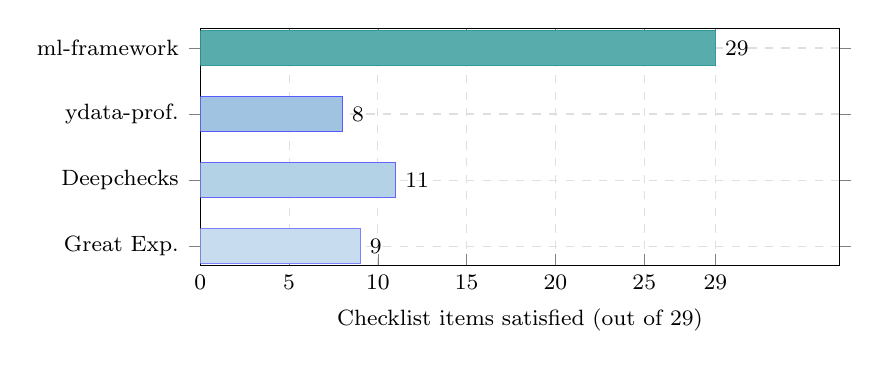
\begin{tikzpicture}
  \begin{axis}[
    xbar, width=0.8\textwidth, height=4.6cm, bar width=0.44cm,
    symbolic y coords={Great Exp.,Deepchecks,ydata-prof.,ml-framework},
    ytick={Great Exp.,Deepchecks,ydata-prof.,ml-framework},
    y tick label style={font=\footnotesize},
    xlabel={Checklist items satisfied (out of 29)}, xlabel style={font=\footnotesize},
    xmin=0, xmax=36, xtick={0,5,10,15,20,25,29},
    xticklabel style={font=\footnotesize},
    nodes near coords, every node near coord/.style={font=\footnotesize\bfseries},
    grid=major, grid style={dashed, gray!25},
  ]
  \addplot[bar shift=0pt, fill={rgb,255:red,200;green,220;blue,240}, draw=blue!50] coordinates {(9,Great Exp.)};
  \addplot[bar shift=0pt, fill={rgb,255:red,180;green,210;blue,230}, draw=blue!60] coordinates {(11,Deepchecks)};
  \addplot[bar shift=0pt, fill={rgb,255:red,160;green,195;blue,225}, draw=blue!65] coordinates {(8,ydata-prof.)};
  \addplot[bar shift=0pt, fill=teal!65, draw=teal!80] coordinates {(29,ml-framework)};
  \end{axis}
  \end{tikzpicture}

  \vspace{0.3em}
  \begin{itemize}\footnotesize
    \item The 29-item checklist is a \textbf{cross-tool comparison instrument} (more granular than the 20-check pipeline; the two numbers measure different things).
    \item \textbf{Fairness note}: the baselines target profiling/validation, not leakage --- the comparison measures \emph{scope}, and the checklist was published with the benchmark code for scrutiny.
  \end{itemize}
\end{frame}

% ============================================================ 19
\begin{frame}{Benchmark II: Leakage Detection --- the Decisive Result}
  Four constructed leakage scenarios, each tool run with default configuration:
  \vspace{0.5em}
  \begin{center}\small
  \begin{tabular}{lcccc}
    \toprule
    \textbf{Scenario} & \textbf{ml-framework} & \textbf{ydata} & \textbf{Deepchecks} & \textbf{Great Exp.} \\
    \midrule
    Perfect proxy ($r{=}1.0$)      & \cmark & \xmark & \xmark & \xmark \\
    \rowcolor{tblAltRow}
    Noisy proxy ($r{\approx}0.97$) & \cmark & \xmark & \xmark & \xmark \\
    ID column (100\% cardinality)  & \cmark & \xmark & \xmark & \cmark \\
    \rowcolor{tblAltRow}
    Indirect computed feature      & \cmark & \xmark & \xmark & \xmark \\
    \midrule
    \textbf{Detection rate} & \textbf{4/4} & 0/4 & 0/4 & 1/4 \\
    \bottomrule
  \end{tabular}
  \end{center}
  \vspace{0.6em}
  \begin{itemize}
    \item Great Expectations' single detection required a \textbf{manually authored rule}; ml-framework's four are fully automatic.
    \item This is precisely the gap the thesis set out to fill.
  \end{itemize}
\end{frame}

% ============================================================ 20
\begin{frame}{Live Demo: Streamlit Web Application}
  \begin{columns}[T]
    \begin{column}{0.5\textwidth}
      \textbf{What you will see} (\texttt{titanic.csv}):
      \begin{enumerate}\setlength\itemsep{0.5em}
        \item Upload the CSV, select \texttt{survived} as target.
        \item Pipeline runs live: 20 checks + impact analysis.
        \item Readiness score \textbf{80.6 / B} with per-dimension breakdown.
        \item \texttt{name} and \texttt{boat} flagged with explanations and suggested fixes.
        \item Downloadable HTML report.
      \end{enumerate}
    \end{column}
    \begin{column}{0.46\textwidth}
      \begin{block}{Run it yourself}
        \texttt{streamlit run app/app.py}
      \end{block}
      \vspace{0.6em}
      \footnotesize Seven tabs: overview, quality, leakage, features, sufficiency, impact, readiness summary.
      \vspace{0.8em}

      \footnotesize\textit{(Backup: pre-recorded capture and generated HTML report, in case of demo issues.)}
    \end{column}
  \end{columns}
\end{frame}

% ============================================================ 21
\begin{frame}{Conclusions}
  \begin{enumerate}\setlength\itemsep{0.7em}
    \item Dataset quality assessment and leakage detection \textbf{can be automated end-to-end}: one config + one CSV $\rightarrow$ scored, explained, actionable verdict.
    \item The \textbf{unified Leakage Risk Score} detects leaks that no single statistic catches, with ablation-backed weights --- \textbf{4/4} benchmark scenarios vs.\ 0--1/4 for existing tools.
    \item \textbf{Semantic analysis with LLMs} extends detection to leakage that is invisible to statistics; the evaluation harness is built and validated, live-model evaluation is queued.
    \item The framework found \textbf{real, previously unflagged issues} in classic public datasets (Titanic \texttt{boat}/\texttt{name}, Wine Quality duplicates).
  \end{enumerate}
  \vspace{0.4em}
  \centering\footnotesize
  Engineering: 17 phases $\cdot$ 14 modules $\cdot$ \textbf{325/325 tests passing} $\cdot$ 3 interfaces $\cdot$ plugin system
\end{frame}

% ============================================================ 22
\begin{frame}{Future Work}
  \begin{enumerate}\setlength\itemsep{0.8em}
    \item \textbf{Live LLM evaluation} of the semantic module against the 30-feature benchmark (top priority --- harness is ready, only credentials are missing).
    \item \textbf{Broader leakage taxonomy}: group leakage, preprocessing leakage (scaler fit on full data), cross-validation contamination.
    \item \textbf{CI/CD integration}: readiness score as a merge gate for data pipelines (the SDK already makes this a few lines of code).
    \item \textbf{Learning thresholds from data}: replacing fixed flagging thresholds with calibrated, dataset-size-aware values.
  \end{enumerate}
\end{frame}

% ============================================================ 23
\begin{frame}
  \begin{center}
    {\LARGE\bfseries\textcolor{upmBlue}{Thank you}}\\[1.2em]
    {\large Questions?}\\[2em]
    \begin{tabular}{rl}
      \textbf{Code:} & \texttt{github.com/jaimecano12/ml-framework} \\[0.3em]
      \textbf{Author:} & Jaime Cano Moraño \\[0.3em]
      & \footnotesize ETSIT-UPM $\cdot$ Illinois Institute of Technology \\
    \end{tabular}
  \end{center}
\end{frame}

\end{document}
